\documentclass[tikz,border=4pt]{standalone}

\usetikzlibrary{positioning,fit,arrows.meta,backgrounds,calc}
\begin{document}
\sffamily\small
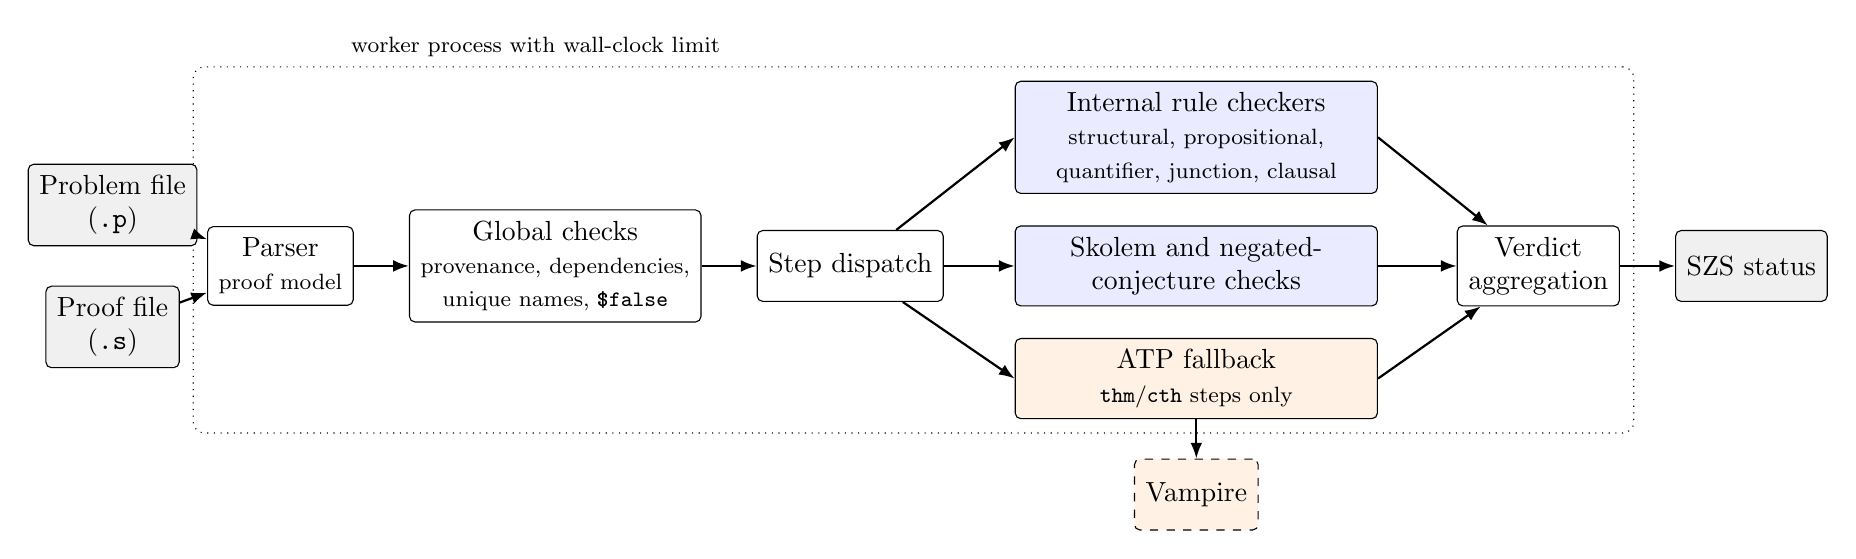
\begin{tikzpicture}[
  node distance=5mm and 7mm,
  box/.style={draw, rounded corners=2pt, align=center, minimum height=9mm, inner sep=4pt, fill=white},
  io/.style={box, fill=gray!12},
  ext/.style={box, dashed, fill=orange!10},
  arr/.style={-{Latex[length=2mm]}, thick},
]
  % inputs
  \node[io] (prob) {Problem file\\(\texttt{.p})};
  \node[io, below=of prob] (proof) {Proof file\\(\texttt{.s})};

  % pipeline
  \node[box, right=12mm of $(prob)!0.5!(proof)$] (parser) {Parser\\ \footnotesize proof model};
  \node[box, right=of parser] (global) {Global checks\\ \footnotesize provenance, dependencies,\\ \footnotesize unique names, \texttt{\$false}};
  \node[box, right=of global] (dispatch) {Step dispatch};

  % checkers
  \node[box, right=9mm of dispatch, fill=blue!8, minimum width=4.6cm] (skolem) {Skolem and negated-\\conjecture checks};
  \node[box, above=4mm of skolem, fill=blue!8, minimum width=4.6cm] (rules) {Internal rule checkers\\ \footnotesize structural, propositional,\\ \footnotesize quantifier, junction, clausal};
  \node[box, below=4mm of skolem, fill=orange!10, minimum width=4.6cm] (atp) {ATP fallback\\ \footnotesize \texttt{thm}/\texttt{cth} steps only};
  \node[ext, below=of atp] (vampire) {Vampire};

  % verdict
  \node[box, right=10mm of skolem] (verdict) {Verdict\\aggregation};
  \node[io, right=of verdict] (szs) {SZS status};

  % worker frame
  \begin{scope}[on background layer]
    \node[draw, dotted, rounded corners=4pt, inner sep=5pt, fit=(parser) (global) (dispatch) (rules) (atp) (verdict),
          label={[font=\footnotesize]above left:worker process with wall-clock limit}] (worker) {};
  \end{scope}

  \draw[arr] (prob) -- (parser);
  \draw[arr] (proof) -- (parser);
  \draw[arr] (parser) -- (global);
  \draw[arr] (global) -- (dispatch);
  \draw[arr] (dispatch) -- (rules.west);
  \draw[arr] (dispatch) -- (skolem);
  \draw[arr] (dispatch) -- (atp.west);
  \draw[arr] (atp) -- (vampire);
  \draw[arr] (rules.east) -- (verdict);
  \draw[arr] (skolem) -- (verdict);
  \draw[arr] (atp.east) -- (verdict);
  \draw[arr] (verdict) -- (szs);
\end{tikzpicture}
\end{document}
